\chapter{Исполнительные электромагнитные механизмы}

\textit{Исполнительным электромагнитным механизмом (ИЭММ)} называется устройство, предназначенное для перемещения рабочего органа в соответствии с сигналами, поступающими от управляющего устройства, и приводимое в движение электромагнитом (ЭМ) с подвижным ферромагнитным элементом. 

Таким образом, ИЭММ служат для преобразования электрического тока в механическое перемещение с целью воздействия на регулирующий орган объекта управления. Они являются наиболее распространенными преобразователями электрического сигнала в механическое перемещение. ИЭММ отличаются большим разнообразием конструктивных решений и благодаря своим богатым функциональным возможностям нашли широкое применение в современной технике (авиационной, ракетной), особенно приборостроении и его специальных отраслях, радиоэлектронной аппаратуре. 

Можно выделить следующие устройства, построенные на ИЭММ:
\begin{itemize}
\item устройства для управления клапанами, вентилями, задвижками, золотниками;
\item устройства для создания удерживающей или тормозящей сил (переключающие, стопорные, зажимные, тормозные, арретирующие);
\item коммутационные устройства электроавтоматики, телефонии, телеметрии (реле коммутационные, токовые, напряжения, контакторы, магнитные пускатели, шаговые переключатели);
\item управляемые электромагнитные муфты, служащие для включения и отключения исполнительных механизмов, их реверса, регулирования скорости, ограничения момента (муфты электромагнитные фрикционные, кулачковые, порошковые, комбинированные);
\item электромагнитные шаговые приводы, электромагнитные устройства вибрационного и ударного действия.
\end{itemize}

\begin{flushleft}
\textbf{Классификация ИЭММ}
\end{flushleft}

ИЭММ классифицируют по назначению, особенностям конструкции, роду тока и другим признакам. В зависимости от рода питающего тока различают три основные группы ИЭММ:
\begin{itemize}
\item ИЭММ постоянного тока нейтральные, они питаются постоянным током, а их действие не зависит от направления тока;
\item ИЭММ постоянного тока поляризованные, их действие зависит от направления тока; 
\item ИЭММ переменного тока, питающиеся переменным током.
\end{itemize}

В приборах чаще всего находят применение ИЭММ постоянного тока нейтральные. ИЭММ постоянного тока в сравнении с ИЭММ переменного тока при прочих равных условиях имеют значительно меньшие массу, габариты, потребляемую мощность, больший коэффициент полезного действия, способны развивать большие тяговые усилия или движущие моменты, имеют более высокую стабильность параметров, конструктивно проще и дешевле.

Кроме того, в ИЭММ переменного тока тяговые усилия имеют импульсный характер, что нежелательно и может привести к нарушению нормальной работы устройства; они менее технологичны в производстве в сравнении с ИЭММ постоянного тока и обычно используются в стационарных промышленных установках, питающихся от сети переменного тока (частотой 50 Гц) достаточной мощности, когда многие их недостатки не являются особым препятствием для применения. Даже в тех приборных устройствах, в которых имеется лишь питающая сеть переменного тока, чаще бывает выгоднее установить специальный выпрямитель, чем использовать ИЭММ переменного тока.

В электромагнитах переменного тока питание обмотки осуществляется от источника переменного тока. Магнитный поток, создаваемый обмоткой, по которой проходит переменный ток, периодически изменяется по величине и направлению (переменный магнитный поток), в результате чего сила электромагнитного притяжения пульсирует от нуля до максимума с удвоенной частотой по отношению к частоте питающего тока. Поэтому ИЭММ переменного тока применяются в различных приборах и системах, использующих данный эффект. 

Например, на применении ИЭММ переменного тока построены все виброустройства, испытательные вибростенды, некоторые электробытовые приборы (например, электробритвы). Рассматривая работу электромагнитных виброустройств, можно выделить их главное преимущество~--- плавное регулирование колебаний, которое происходит за счет изменения электрического тока в обмотке.

\begin{flushleft}
\textbf{Структура ИЭММ. ИЭММ как преобразователь энергии }
\end{flushleft}

Несмотря на многообразие выполняемых функций и конструктивных решений, в любом ИЭММ можно выделить две основные части: электромагнит (ЭМ), который играет роль двигателя, и передаточный механизм (ПМ). 

Конструкция некоторых ИЭММ представлена на рис.~\ref{pic:9IEMM}~а; \ref{pic:9strongIEMM}~а; \ref{pic:9step}~а, а их схемы~--- соответственно на рис.~\ref{pic:9IEMM}~б; \ref{pic:9strongIEMM}~б; \ref{pic:9step}~б.

\begin{figure}[h!]
	\caption{ Пример конструкции ИЭММ: электромагнитное реле (а) и схема работы (б) }
	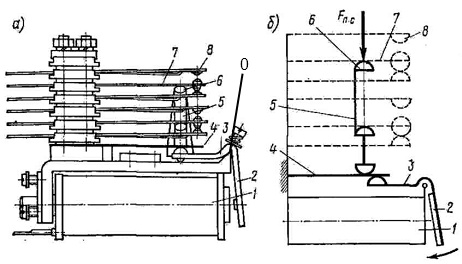
\includegraphics[width=1\textwidth]{9IEMM.png}
	\label{pic:9IEMM}
\end{figure}

На рис.~\ref{pic:9IEMM}~а,~б изображено электромагнитное реле, электромагнит которого отмечен позицией 1. ПМ (передаточный механизм)  в нем состоит из двуплечего рычага 3, одним из плеч которого служит якорь 2 ЭМ, и тангенсной передачи, где коромыслом является другое плечо рычага 3, а толкателем~-- гребенка 5. При включении реле подвижный элемент (ПЭ)~-- якорь 2, поворачиваясь относительно ножевой опоры 0, своим плечом 3 перемещает конечный элемент (КЭ)~-- гребенку 5, которая своими упорами 6, преодолевая силу сопротивления контактных пружин 7 (силу полезной нагрузки устройства) и плоской возвратной пружины 4, изгибает их до замыкания контактов 8 (элемент нагрузки~-- контактные пружины~-- на схеме изображен штриховыми линиями). После отключения реле ПЭ якорь 2 возвращается в исходное положение пружиной~4.

\begin{flushleft}
\textbf{ Силовой ИЭММ }
\end{flushleft}

На рис.~\ref{pic:9strongIEMM}~а,~б показан силовой ИЭММ. Якорь~2 его ЭМ~1 играет роль ползуна кривошипно-ползунной передачи, в которой кривошипом является участок ОВ зубчатого сектора~3, а ползуном~-- якорь. Кроме этой передачи в состав ПМ (передаточный механизм) входит также зубчатая передача сектор~3~-- трибка~4. При включении устройства якорь~2, втягиваясь в ЭМ, тянет за рычаг ВС, который, в свою очередь, заставляет поворачиваться сектор~3 и в конечном счете приводит к повороту элемента ПМ на оси трибки~4. При этом преодолевается момент полезного сопротивления $ M_\text{пс} $ устройства, приложенный к этой оси. В исходное положение ПМ (передаточный механизм) устанавливается после отключения ЭМ винтовой пружиной~5. (Трибка, мелкомодульное зубчатое колесо с малым числом зубьев (6~-- 16), составляющее одно целое со своей осью вращения).

\begin{figure}[h!]
	\caption{ Пример конструкции ИЭММ: силовой ИЭММ (а) и схема работы (б) }
	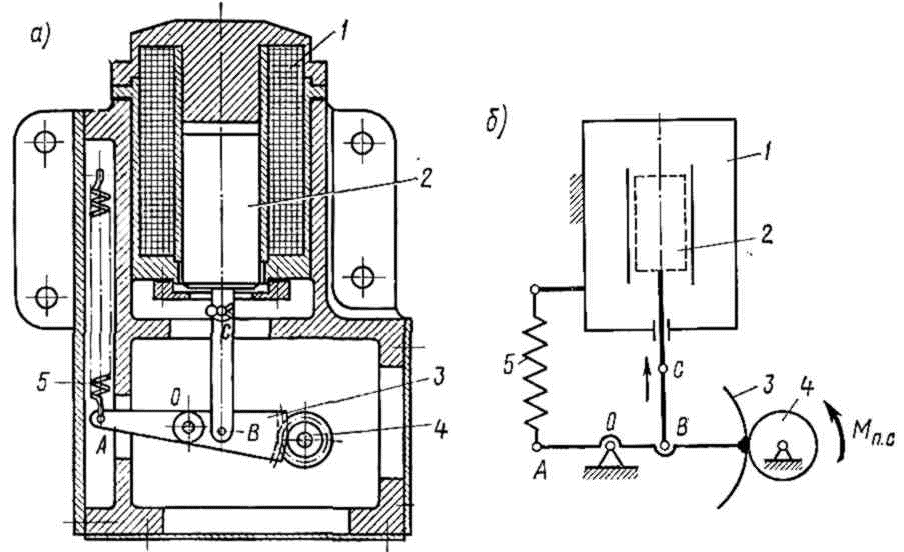
\includegraphics[width=1\textwidth]{9strongIEMM.png}
	\label{pic:9strongIEMM}
\end{figure}

\begin{figure}[h!]
	\caption{ Пример конструкции ИЭММ: шаговое поворотное устройство(а) и схема работы (б) }
	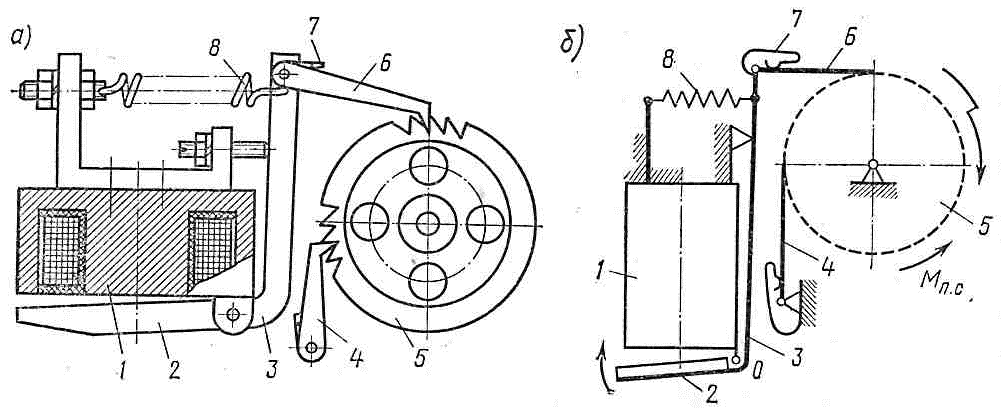
\includegraphics[width=1\textwidth]{9step.png}
	\label{pic:9step}
\end{figure}

\begin{flushleft}
\textbf{Шаговое поворотное устройство}
\end{flushleft}
 
На рис.~\ref{pic:9step}~а,~б представлено шаговое поворотное устройство. Его ПМ (передаточный механизм) представляет собой совокупность двуплечего рычага~3, одно из плеч которого, как и в случае электромагнитного реле, является ПЭ (подвижный элемент) ЭМ~1 и храповой передачи, состоящей из храпового колеса~5, рабочей~6 и стопорной~4 собачек с прижимными пружинами~7. 

При включении ЭМ~1 его ПЭ~2 поворачивается относительно опоры О. Это движение передается рычагом~3 рабочей собачке~6, которая поворачивает храповое колесо~5 на определенный угол. В исходное положение ПМ возвращается пружиной~8. Стопорная собачка~4 не препятствует повороту храпового колеса~5 при рабочем ходе собачки~6 и фиксирует его при обратном ходе этой собачки. Момент нагрузки приложен к КЭПМ (конечный элемент ПМ)~-- оси храпового колеса.

Обязательным элементом любого ИЭММ с нейтральным ЭМ, как это следует из рис.~\ref{pic:9IEMM}$ \ldots $\ref{pic:9step}, является возвратная пружина. При включении ИЭММ она создает сопротивление в дополнение к силам нагрузки, а при отключении работает как движущий элемент.

Структурная схема любого ИЭММ может быть представлена, как показано на рис.~\ref{pic:9struct}. Входной ток $ i $ ЭМ возбуждает силу электромагнитного притяжения $ F_\text{э} $, действующую на ПЭ (подвижный элемент), движение которого преобразуется затем в ПМ (передаточный механизм) в поступательное $ x $ или угловое перемещение $ \varphi $ его КЭ (конечный элемент). Последний совершает механическую работу по преодолению сил $ F_\text{пс} $ или моментов $ M_\text{пс} $ полезного сопротивления, т.е. полезной нагрузки, приложенной к этому элементу.

\begin{figure}[h!]
	\caption{ Структурная схема ИЭММ }
	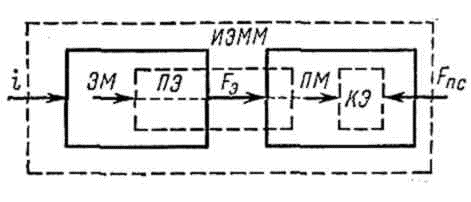
\includegraphics[width=0.6\textwidth]{9struct.png}
	\label{pic:9struct}
\end{figure}

В отличие от исполнительного электромеханического привода, в котором ПМ, как правило, представляет собой передачу зубчатыми колесами, ПМ в ИЭММ отличается большим разнообразием, что частично проиллюстрировано схемами рис.~\ref{pic:9IEMM}$ \ldots $\ref{pic:9step}. Более того, ПМ в ИЭММ может вовсе отсутствовать, при этом роль КЭ (конечный элемент), к которому прикладывается нагрузка, выполняет ПЭ (подвижный элемент) ЭМ (например, в устройствах типа электромагнитных клапанов и муфт).

ИЭММ может также рассматриваться как некоторый преобразователь энергии, что поясняется схемой рис.~\ref{pic:9energy}. 

Электрическая энергия $ W_\text{э} $ на входе ЭМ, полученная от источника тока, претерпевает в ЭМ преобразование в магнитную энергию, которая затем преобразуется в механическую энергию $ W_\text{м} $ ПЭ ЭМ, а последняя в ПМ (передаточный механизм) переходит в полезную механическую энергию $ W_0 $, связанную с движением КЭ ПМ. В обеих частях ИЭММ происходят потери энергии: в ЭМ~-- $ W_\text{эп} $, а в ПМ~-- $ W_\text{мп} $. $ W_\text{эп} $ обусловливается потерями в омическом сопротивлении обмотки ЭМ, потерями на перемагничивание магнитного материала ЭМ и на вихревые токи; $ W_\text{мп} $ связана с преодолением сил вредного сопротивления в ПМ, т.е. сил трения.

\begin{figure}[h!]
	\caption{ ИЭММ как преобразователь энергии}
	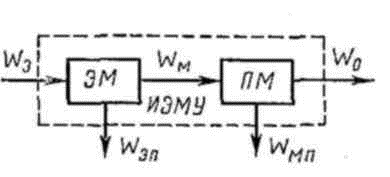
\includegraphics[width=0.6\textwidth]{9energy.png}
	\label{pic:9energy}
\end{figure}

\begin{flushleft}
\textbf{Элементы магнитной цепи и основные элементы ЭМ}
\end{flushleft}

\textit{ЭМ} --- это устройство, работа которого основана на взаимодействии подвижного ферромагнитного элемента с магнитным полем намагничивающей обмотки.

Рассмотрим элементы магнитной цепи и основные элементы ЭМ на примере конструктивной схемы, часто встречающейся у электромагнитных реле (рис.~\ref{pic:9EMrele}).

\begin{figure}[h!]
	\caption{ Элементы магнитной цепи ЭМ реле}
	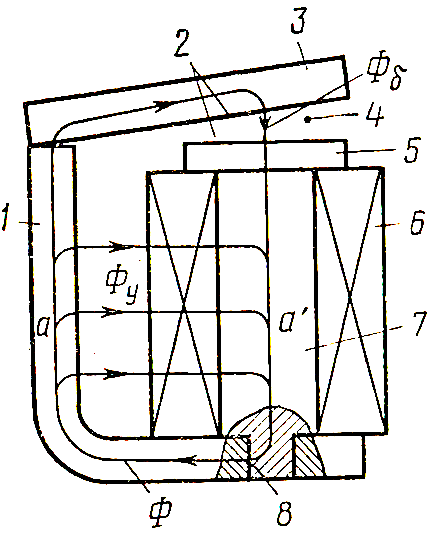
\includegraphics[width=0.45\textwidth]{9EMrele.png}
	\label{pic:9EMrele}
\end{figure}

\textit{Магнитная цепь}~--- это совокупность всех элементов, через которые замыкается магнитный поток. Она включает участки, выполненные из ферромагнитных материалов, и воздушные зазоры.

Конструктивно ЭМ состоит из двух основных частей: катушки с расположенной на ней обмоткой~6 (ЭМ может иметь несколько катушек и несколько обмоток) и магнитопровода~-- элементов из ферромагнитных материалов. Обмотка в ЭМ служит для создания намагничивающего поля, а магнитопровод~-- для его усиления и проведения результирующего магнитного потока. Магнитопровод включает подвижный элемент~3, называемый якорем, и неподвижную часть. Неподвижная часть в зависимости от конструктивного исполнения и формы может носить разные названия, причем состоять из нескольких деталей (основания, корпуса, фланцев).

На рис.~\ref{pic:9EMrele} элементы неподвижной части имеют следующие названия: 1~-- ярмо (корпус, скоба), 5~-- полюсный наконечник или шляпка, 7~-- сердечник. Сердечником называют часть магнитопровода, находящуюся внутри катушки. Иногда роль сердечника выполняет якорь. Якорь отделяется от остальных частей магнитопровода воздушными зазорами и представляет собой элемент ЭМ, который, воспринимая электромагнитную силу, передает ее ведущему элементу ПМ (передаточный механизм) ИЭММ. 

Количество и форма воздушных зазоров, отделяющих якорь от неподвижной части магнитопровода, зависят от конструкции ЭМ. Воздушные зазоры, в которых возникает полезная сила, называют рабочими (4 на рис.~\ref{pic:9EMrele}); зазоры, в которых не возникают силы в направлении возможного перемещения якоря, называют паразитными (8 на рис.~\ref{pic:9EMrele}). Паразитные зазоры обусловлены технологическими факторами, а также необходимостью исключения залипания якоря от остаточной намагниченности при отключении ЭМ. Их размер колеблется от сотых до десятых долей миллиметра.

Часть полного магнитного потока $ \Phi $, которая проходит через рабочий зазор $ \delta $, называется рабочим магнитным потоком и обозначается $ \Phi_\delta $. Часть потока $ \Phi $, которая не замыкается через рабочий зазор, называется потоком рассеяния или потоком утечки и обозначается $ \Phi_s $ или $ \Phi_\text{у} $. Поверхности магнитопровода, ограничивающие рабочий зазор, называют полюсами~2.

\section{Основные характеристики ЭМ}
\begin{flushleft}
\textbf{Механическая характеристика или характеристика противодействующих сил (нагрузки)}
\end{flushleft}
Это зависимость полной силы (момента) сопротивления, приведенной к якорю, от его положения или размера рабочего зазора: $ F_\text{п} = F_\text{п}(\delta) $. Силы сопротивления включают силы полезного сопротивления (полезной нагрузки), приложенные к конечному элементу (КЭ) передаточного механизма (с ними связано выполнение полезной работы), а также силы вредного сопротивления, к которым относятся силы трения, действующие на подвижные элементы ПМ (передаточный механизм), и сила возвратной пружины. Типичные характеристики нагрузок изображены на рис.~\ref{pic:9charact}~а$ \ldots $г.

\begin{figure}[h!]
	\caption{ Типичные характеристики нагрузок }
	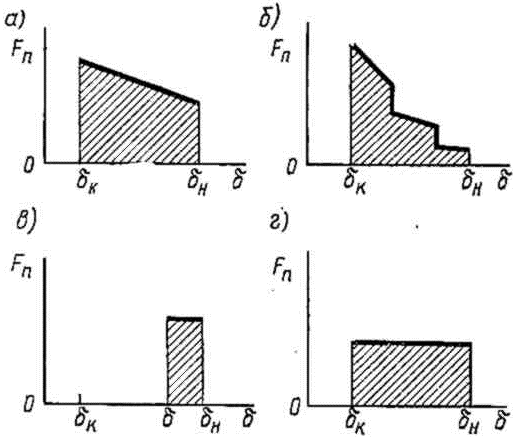
\includegraphics[width=0.6\textwidth]{9charact.png}
	\label{pic:9charact}
\end{figure}

\begin{flushleft}
\textbf{Тяговая характеристика}
\end{flushleft}
Это зависимость электромагнитной силы притяжения, действующей на якорь, от его положения или размера рабочего зазора $ F_\text{э} = F_\text{э}(\delta) $. Различают статическую тяговую характеристику, если она рассматривается при постоянных значениях питающего тока (или напряжения), т.е. при $ I = const $ (или $ U = const $), и динамическую тяговую характеристику, учитывающую в отличие от статической изменение тока в обмотке ЭМ при движении якоря. В силу разного характера изменения тока в режиме включения и отключения ИЭММ динамические тяговые характеристики для этих режимов также различны. Взаимное расположение тяговых и механических характеристик показано на рис.~\ref{pic:9mech}.

\begin{figure}[h!]
	\caption{ Типичные характеристики нагрузок }
	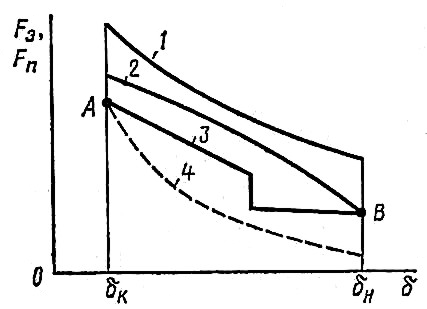
\includegraphics[width=0.6\textwidth]{9mech.png}
	\label{pic:9mech}
\end{figure}

Для надежного срабатывания ИЭММ при включении необходимо, чтобы динамическая тяговая характеристика~2 во всем диапазоне изменения зазора   проходила выше механической характеристики 3, а для четкого срабатывания ИЭММ при отключении, наоборот, динамическая характеристика~4 должна проходить ниже механической. 

Обеспечение при расчете ИЭММ необходимого взаимного расположения тяговой и механической характеристик называют их согласованием. Обычно ограничиваются согласованием статической тяговой~1 и механической~3 характеристик, поскольку построение динамической тяговой характеристики связано с определенными трудностями. При этом учитывают то обстоятельство, что динамическая тяговая характеристика~4 лежит ниже статической~1.

\begin{flushleft}
\textbf{Нагрузочная характеристика электромагнита}
\end{flushleft}
Эта характеристика связывает значение электромагнитной силы и величину напряжения, подведенного к обмотке, или тока в ней при фиксированном положении якоря:
\[ F_\text{э} = f(u),\, F_\text{э} = f(i)\;\text{при}\; \delta = const.\]

\begin{flushleft}
\textbf{Характеристики нагрева}
\end{flushleft}

Это зависимость температуры нагрева обмотки ЭМ от продолжительности включенного состояния $ \nu = \nu (t) $.

\begin{flushleft}
\textbf{Коэффициент запаса}
\end{flushleft}
Отношение установившегося значения силы тока, к  силе тока срабатывания (при которой происходит срабатывание электромагнита) носит название коэффициента запаса: 
\[ k_\text{з} = \dfrac{I_y}{I_\text{ср}}. \]

Коэффициент запаса электромагнита по условиям надежности всегда выбирается больше единицы.

\begin{flushleft}
\textbf{Прочие характеристики и параметры: масса, габариты, потребляемая мощность, показатели эффективности}
\end{flushleft}

\section{Конструктивные типы ЭМ и их особенности}
Существующие в настоящее время ЭМ характеризуются большим разнообразием конструктивных форм магнитопровода, количеством и расположением катушек. Их классифицируют по следующим наиболее важным признакам:
\begin{itemize}
\item по характеру движения якоря:
\begin{itemize}
\item с прямоходовым якорем;
\item с поворотным якорем;
\end{itemize}
\item по форме магнитопровода:
\begin{itemize}
\item Ш-образным;
\item U-образным;
\item подковообразным;
\item цилиндрическим;
\end{itemize} 
\item по расположению якоря относительно намагничивающей обмотки:
\begin{itemize}
\item с внутренним, или втягивающимся, якорем, который в этом случае иногда называют плунжером;
\item и с внешним, или притягивающимся, якорем:
\begin{itemize}
\item ЭМ с внешним притягивающимся якорем, у которых якорь движется в направлении магнитного потока $ \Phi_\delta $;
\item ЭМ с якорем, движущимся поперек направления потока $ \Phi_\delta $.
\end{itemize}
\end{itemize} 
\end{itemize}

ЭМ с втягивающимся якорем называют иногда соленоидными или плунжерными, а ЭМ с внешним притягивающимся якорем~--- ЭМ клапанного типа.

Основные конструктивные типы ЭМ изображены на рис.~\ref{pic:9construct}. ЭМ с втягивающимся якорем (рис.~\ref{pic:9construct}~а,~б,~в) могут развивать большие усилия и иметь ход якоря, изменяющийся в очень большом диапазоне. Они экономичны, отличаются  хорошей технологичностью и получили широкое распространение. ЭМ клапанного типа (рис.~\ref{pic:9construct}~г,~д,~е) характеризуются достаточно большими усилиями, но применяются при сравнительно небольших ходах якоря, отличаются высоким быстродействием, получили широкое распространение, особенно в коммутационных устройствах. ЭМ с якорем, движущимся поперек направления потока $ \Phi $ (рис.~\ref{pic:9construct}~ж,~з), развивают небольшие усилия, но позволяют путем соответствующего согласования форм полюсов получить сложный вид тяговой характеристики. Они малоэкономичны и обладают невысоким быстродействием.

\begin{figure}[h!]
	\caption{ Типичные характеристики нагрузок }
	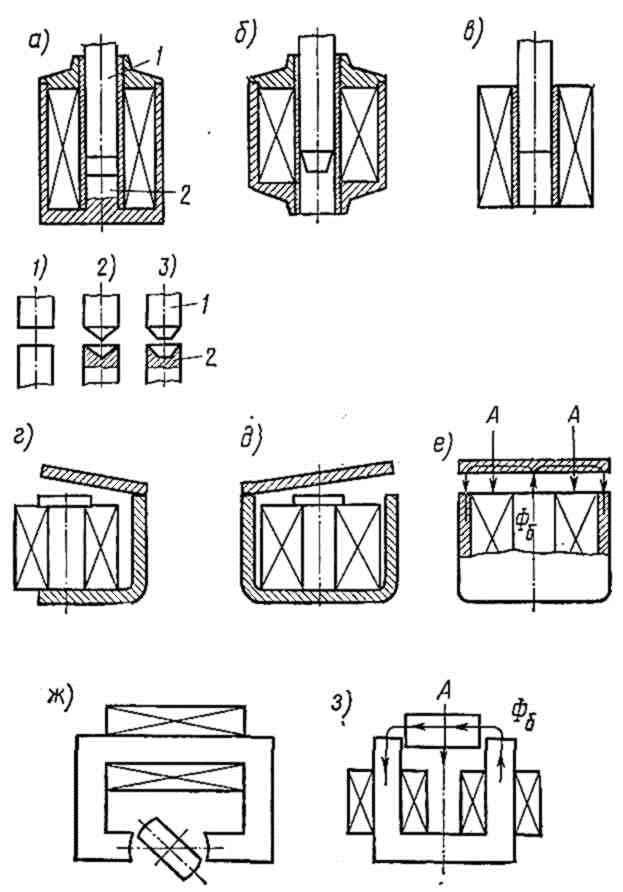
\includegraphics[width=0.6\textwidth]{9construct.png}
	\label{pic:9construct}
\end{figure}

\section{Основные уравнения рабочего процесса ИЭММ}

При описании работы ИЭММ удобно расчленить его на три физически отличные друг от друга, но связанные между собой подсистемы: электрическую, магнитную и механическую. Электрическая подсистема включает в себя электрическую цепь намагничивающей обмотки, магнитная~-- магнитопровод, а механическая~-- передаточный механизм вместе с якорем ЭМ~-- ведущим элементом этого механизма. Ниже приведены основные уравнения, описывающие рабочий процесс в ИЭММ.

\textit{Уравнение электрической подсистемы} (цепи обмотки ЭМ):
\[ U = iR + \dfrac{d\psi}{dt},\]
где $ U $ -- напряжение источника питания цепи обмотки; $ R $ -- активное сопротивление обмотки; $ i $~-- мгновенное значение тока в обмотке; $ \psi $~-- мгновенное значение потокосцепления обмотки; $ t $ -- время. Это уравнение позволяет исследовать первый этап энергетического преобразования в ЭМ, т.е. преобразование электрической энергии источника питания в магнитную энергию намагниченности магнитопровода, а также выполнить расчет обмотки.

\textit{Уравнение магнитной подсистемы} (намагничивания магнитопровода):
\[\psi = \psi(i,\delta), \]
устанавливает функциональную связь между током в обмотке $ i $ и рабочим зазором $ \delta $, с одной стороны, и потокосцеплением $ \psi $~-- с другой.

\textit{Уравнение механической подсистемы} (движения якоря):
\[ m\dfrac{d^2 x}{dt^2} - F_\text{э} + F_\text{п}=0, \]
где $ m $ -- приведенная к якорю масса всех движущихся элементов ПМ, $ x $~-- перемещение якоря, $ F_\text{э} $ -- сила электромагнитного притяжения якоря; $ F_\text{п} $ -- сила, противодействующая движению якоря. В этом уравнении $ x = \delta_\text{н} - \delta $, где $ \delta_\text{н} $ и $ \delta $~-- соответственно начальный и текущий размеры рабочего зазора.

Сила $ F_\text{э} $ есть функция перемещения якоря (или размера зазора):
\[ F_\text{э} = \dfrac{dW_m}{dt} = \dfrac{-d}{d\delta}\int\limits_{0}^{\psi_\delta}i\,d\psi,   \]
где $ W_m $ -- полное значение запасенной в ЭМ магнитной энергии, соответствующее зазору $ \delta $, току $ I_\delta $ и потокосцеплению $ \psi_\delta $.

В общем случае сила $ F_\text{п}  = F_\text{п} (x_0,\,\dfrac{dx_\text{пэ}}{dt} ) $ складывается из силы полезного сопротивления (полезной нагрузки) на выходе ПМ, которая является обычно функцией положения конечного элемента ПМ $ x_0 $, и сил вредного сопротивления (сил трения), действующих на подвижные элементы ПМ, которые являются функцией от производных перемещения $ \dfrac{dx_\text{пэ}}{dt} $ этих элементов (все силы сопротивления рассматриваются приведенными к якорю).

К основным уравнениям ИЭММ относят также\textit{ уравнения тепловых процессов} в ЭМ:

уравнение нагрева  $ \nu = \nu (P,\,t_\text{вкл},\,l_1,\,l_2,\ldots,l_n,\,\chi) $, где $ \nu $~-- температура нагрева обмотки ЭМ, как наиболее чувствительного в тепловом отношении элемента ИЭММ; $ P $~-- мощность, выделенная в обмотке; $ t_\text{вкл} $~-- время включенного состояния обмотки; $ l_1,\,l_2,\ldots,l_n $~-- размеры обмотки и элементов магнитопровода; $ \chi $~-- тепловые характеристики материалов ЭМ;

уравнение охлаждения $ \nu = \nu (t_\text{отк},\,l_1,\,l_2,\ldots,l_n,\,\chi ) $, где $ t_\text{отк} $~-- время охлаждения с момента отключения обмотки от сети.

\section{Динамические характеристики и способы повышения быстродействия ИЭММ}

\textbf{Динамические характеристики срабатывания}, определяющие быстродействие ИЭММ, являются важнейшими характеристиками приборных ИЭММ. К ним относятся время срабатывания при включении $ t'_\text{ср} $ и время срабатывания при отключении $ t''_\text{ср} $ ИЭММ.

В зависимости от значений времени срабатывания ИЭММ условно делят на:
\begin{itemize}
\item $ t'_\text{ср} < 50 $ мс -- быстродействующие;
\item $ t'_\text{ср} = 50\ldots150 $ мс -- ИЭММ с нормальным временем действия;
\item $ t'_\text{ср} > 150 $ мс -- ИЭММ замедленного действия.
\end{itemize}

Быстродействие специальных ИЭММ может достигать значения порядка 1 мс.

\textit{Временем срабатывания при включении} называется время с момента включения обмотки до момента полной остановки якоря (будем отождествлять в дальнейшем время срабатывания ИЭММ с временем срабатывания ЭМ).

\textit{Временем срабатывания при отключении} называется время с момента отключения обмотки до момента возврата якоря в начальное положение.

\textit{Время срабатывания} можно разбить на две составляющие:
\begin{itemize}
\item время трогания $ t_\text{тр} $ -- время с момента подачи сигнала на обмотку (на включение или отключение) до начала движения якоря;
\item время движения $ t_\text{дв} $ -- время от начала движения якоря до полной его остановки:
\end{itemize}
\[ t'_\text{ср} = t'_\text{тр} + t'_\text{дв},\, t''_\text{ср} = t''_\text{тр} + t''_\text{дв}.  \]

Здесь один штрих соответствует режиму включения, а два штриха~-- режиму отключения.

Определим время трогания и движения при включении. При включении обмотки на постоянное напряжение переходный процесс в ЭМ определяется известным уравнением переходного процесса
\[ U = iR + \dfrac{d\psi}{dt}, \]
где $ U $ -- напряжение источника питания цепи обмотки, $ i $~-- мгновенное значение тока в обмотке, $ R $~-- сопротивление цепи обмотки, $ \psi $~-- мгновенное значение полного потокосцепления обмотки, $ t $~-- время.

В исходном состоянии ЭМ, когда рабочий зазор равен начальному, магнитопровод, как правило, ненасыщен, т.е. имеет место линейная зависимость $ \psi = iL $, где $ L $~-- индуктивность ЭМ при отпущенном якоре.

Решая уравнение переходного процесса относительно $ dt $, получаем:
\begin{equation}
\label{eq:8tshtrihSR}
t'_\text{ср} = \dfrac{L}{R}\, ln\left( \dfrac{I_\text{уст}}{I_\text{уст} - i'_\text{тр}} \right)
\end{equation}

Здесь индуктивность $ L = \omega^2 G_{\delta\Sigma} $, $ \omega $~-- число витков в обмотке ЭМ, $ G_{\delta\Sigma} $~-- эквивалентная проводимость воздушных зазоров на пути магнитного потока при отпущенном якоре ЭМ,\\ $ I_\text{уст} = U/R $~--– ток в установившемся режиме. 

Ток трогания $ i'_\text{тр} $, т.е. ток, при котором начинается движение якоря, может быть определен из соответствующей формулы для силы притяжения якоря, с учетом того, что при $ i=i'_\text{тр} $ электромагнитная сила притяжения $ F_\text{э} $ равна противодействующей силе $ F_\text{п} $ при начальном воздушном зазоре. Путем соответствующих расчетов можно получить следующее соотношение:
\[ i'_\text{тр} = \dfrac{1}{\omega} \sqrt{\dfrac{2F_\text{п}|_{\delta = \delta_\text{н}}}{\left|\dfrac{dG_{\delta\Sigma}}{d\delta}\right|}}  \]

Для оценки $ t'_\text{дв} $ иногда можно пользоваться упрощенным методом расчета по статическим тяговой и механической характеристикам. Согласно упрощенному методу, учитывается лишь уравнение движения механической подсистемы ИЭММ:
\[ m\dfrac{d^2 x}{dt^2} - F_\text{э} + F_\text{п} = 0. \] 

Допуская, что результирующая сила $ F_\text{э} - F_\text{п} $, действующая на якорь при срабатывании ИЭММ, сохраняется постоянной и независимой от перемещения якоря, путем соответствующих расчетов можно получить следующее соотношение:
\begin{equation}
\label{eq:8tshtrih}
 t'_\text{дв} = \sqrt{2m\dfrac{\delta_\text{н} - \delta_\text{к}}{F_\text{э} - F_\text{п}}}
\end{equation}

Построив на одном рисунке характеристики $ F_\text{э} = F_\text{э}(\delta) $ и $ F_\text{п} = F_\text{п}(\delta) $, затем найдем площадь $ A^* $ (рис.~\ref{pic:9asqure}), ограниченную этими характеристиками при изменении $ \delta $ от $ \delta_\text{н} $  до $ \delta_\text{к} $. 

Тогда с учетом масштабов сил $ \mu_F $ и перемещений $ \mu_\delta $ среднее по ходу якоря значение: 
\[ F_\text{э} - F_\text{п} = A^* \dfrac{\mu_F \mu_\delta}{\delta_\text{н} - \delta_\text{к}}. \]

Подставляя его в уравнение \eqref{eq:8tshtrih} для $ t'_\text{дв} $, окончательно получим
\begin{equation}
\label{eq:8tshtrih1}
t'_\text{дв} = (\delta_\text{н} - \delta_\text{к}) \sqrt{\dfrac{2m}{A^*\mu_F\mu_\delta}}
\end{equation}

Поскольку эта формула не учитывает динамику процесса движения якоря, то расчет по ней $ t'_\text{дв} $ дает ошибку в несколько десятков процентов.

Расчет времени срабатывания ЭМ при отключении $ t''_\text{ср} $ выполняется в принципе теми же методами, что и расчет времени срабатывания при включении $ t'_\text{ср} $.

\begin{figure}[h!]
	\caption{ Типичные характеристики нагрузок }
	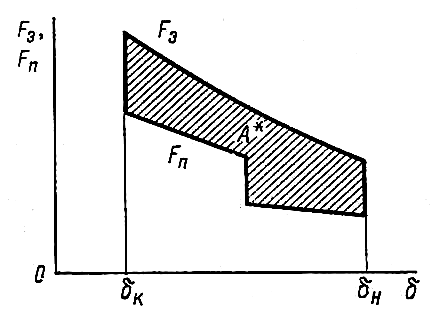
\includegraphics[width=0.6\textwidth]{9asqure.png}
	\label{pic:9asqure}
\end{figure}

Быстродействие ИЭММ можно повысить следующими способами:
\begin{itemize}
\item Выбором рациональной конструктивной схемы ЭМ. Магнитопровод ЭМ желательно выполнять таким, чтобы потоки рассеяния по возможности участвовали в создании силы притяжения и чтобы свести к минимуму размер паразитных зазоров;
\item Всемерным уменьшением вихревых токов в электропроводных частях ЭМ. Наличие вихревых токов при срабатывании ЭМ обусловливается изменением магнитного потока вследствие изменения магнитного сопротивления ему при изменении рабочего зазора. Вихревые токи замыкаются в плоскостях, параллельных плоскостям токов намагничивающей обмотки. 

Вихревые токи могут быть уменьшены путем выбора соответствующего материала магнитопровода с целью уменьшения потерь на перемагничивание, а также путем  выполнения магнитопровода наборным из отдельных пластин (шихтованным), применением для магнитопровода материалов с высоким удельным электрическим сопротивлением (кремнистых сталей), использованием разрезов на возможных путях вихревых токов; при этом недопустимо применение неразрезных металлических каркасов катушек, направляющих втулок якоря-сердечника в соленоидных ЭМ.
\item Уменьшением хода якоря  , массы подвижных частей ИЭММ (и в первую очередь массы m якоря) и противодействующих сил (что соответствует увеличению площади $ A^* $ в приближенной формуле \eqref{eq:8tshtrih1}); все это следует из формулы \eqref{eq:8tshtrih1}.
\item Увеличением подводимой мощности к ЭМ (увеличением напряжения питания $ U $ или уменьшением сопротивления $ R $ обмотки); это вытекает из формулы \eqref{eq:8tshtrihSR} для $ t'_\text{ср} $. Однако при этом необходимо учитывать, что коэффициент запаса можно увеличивать только в пределах индукции насыщения материала магнитопровода.
\end{itemize}

Если перечисленные способы не позволяют достичь желаемого результата, то можно использовать форсирование ЭМ, т.е. повышение подводимой мощности только во время срабатывания ИЭММ.

\begin{figure}[h!]
	\caption{ Типичные характеристики нагрузок }
	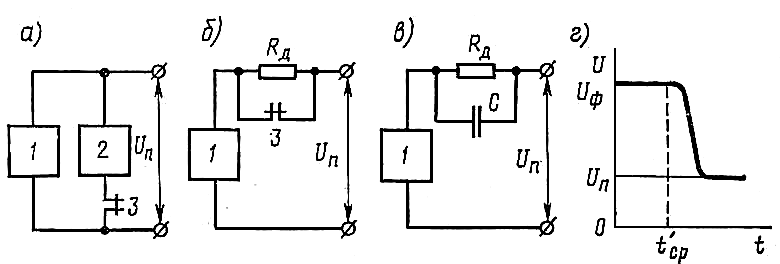
\includegraphics[width=1\textwidth]{9dopobmotka.png}
	\label{pic:9dopobmotka}
\end{figure}

Форсирование можно достичь:
\begin{itemize}
\item применением дополнительной обмотки~2, которая после срабатывания ИЭММ отключается от источника питания его же нормально-замкнутыми контактами~3 (рис.~\ref{pic:9dopobmotka}~а), позиция 1 на нем~-- основная намагничивающая обмотка;
\item шунтированием нормально-замкнутым контактом~3 ИЭММ добавочного сопротивления $ R_\text{д} $, включенного последовательно с намагничивающей обмоткой (рис.~\ref{pic:9dopobmotka}~б); при срабатывании намагничивающий ток определяется только сопротивлением обмотки, после срабатывания ток становится меньше вследствие подключения  $ R_\text{д} $, но все же он достаточен для удержания якоря в притянутом положении;
\item использованием $ RC $-цепочки (рис.~\ref{pic:9dopobmotka}~в); конденсатор в этой схеме~-- своего рода контакт, как в схеме рис.~\ref{pic:9dopobmotka}~б, но с плавным подключением $ R_\text{д} $ ; в начальный момент, когда конденсатор незаряжен, весь ток устремляется через него, т.е. мимо $ R_\text{д} $, по мере заряда конденсатора часть тока начинает проходить через $ R_\text{д} $, а когда он полностью зарядится, ток идет только через $ R_\text{д} $, причем он меньше, чем в начальный момент включения; $ t'_\text{ср} $ получается минимальным при определенном соотношении между параметрами электрической цепи ($ C,\, R,\, R_\text{д},\, L $);
\end{itemize} 

применением специальных электронных форсирующих схем питания, обеспечивающих в момент срабатывания напряжение питания, превышающее напряжение питания $ U_\text{п} $ ЭМ во включенном состоянии (рис.~\ref{pic:9dopobmotka}~г).

Повышение быстродействия ИЭММ путем форсирования ЭМ достигается ухудшением прочих характеристик ИЭММ: в первом случае увеличиваются масса и габариты ЭМ от дополнительной обмотки, во втором~-- повышается энергопотребление ИЭММ вследствие падения мощности на добавочном сопротивлении; в третьем~-- требуется конденсатор большой емкости, что приводит к увеличению массы и габаритов устройства; в четвертом~-- эти характеристики также ухудшаются из-за применения специальной электронной схемы питания. При любом способе форсирования ЭМ снижается надежность ИЭММ. 

\begin{flushleft}
\textbf{Особенности расчета ИЭММ}
\end{flushleft}

Специфика и сложность расчета ИЭММ связаны в основном с наличием в нем электромагнита, расчет которого существенно отличается от расчета механических элементов приборов. Расчет последних, как известно, выполняется по сравнительно простым и точным формулам практически в один прием. Что же касается расчета ЭМ, то он не может быть выполнен в один прием, поскольку информации, необходимой для расчета, как правило, в этом случае недостаточно и приходится на первых порах при определении основных характеристик задаваться другими расчетными характеристиками и по ходу расчета неоднократно проверять, насколько удачно приняты значения этих характеристик, насколько они отвечают требованиям задания, и при необходимости часть расчета или даже полностью весь расчет повторять.

Основные исходные данные, необходимые для проектирования ИЭММ, устанавливаются требованиями технического задания. 

